\documentclass[border=5pt]{standalone}
\usepackage{tikz}
\usepackage{amsmath}
\usepackage{fontspec}
\usetikzlibrary{arrows.meta,calc}

\newfontfamily\figurefont[
  Path=assets/fonts/,
  UprightFont=AlphaLyrae-Medium.ttf,
  BoldFont=AlphaLyrae-Medium.ttf,
  BoldFeatures={FakeBold=1.6},
  Ligatures=TeX,
  RawFeature=-calt
]{Alpha Lyrae}

\definecolor{ink}{HTML}{243142}
\definecolor{vision}{HTML}{2E86AB}
\definecolor{model}{HTML}{E8871E}
\definecolor{policy}{HTML}{7FB069}

\begin{document}
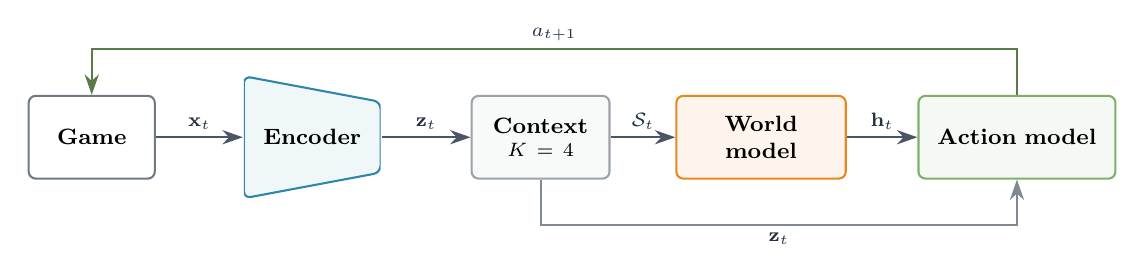
\begin{tikzpicture}[
  font=\figurefont\footnotesize,
  box/.style={
    rounded corners=2.5pt,
    draw=ink!65,
    line width=0.75pt,
    fill=white,
    minimum height=1.05cm,
    align=center,
    inner xsep=5pt,
    inner ysep=5pt,
    font=\figurefont\footnotesize
  },
  encoderbox/.style={
    box,
    draw=none,
    fill=none,
    rounded corners=0pt,
    minimum height=1.55cm,
    inner xsep=7pt,
    path picture={
      \path[
        draw=vision,
        fill=vision!7,
        line width=0.75pt,
        rounded corners=2.5pt,
        line join=round
      ]
        (path picture bounding box.north west) --
        ($(path picture bounding box.east)!0.58!(path picture bounding box.north east)$) --
        ($(path picture bounding box.east)!0.58!(path picture bounding box.south east)$) --
        (path picture bounding box.south west) -- cycle;
    }
  },
  contextbox/.style={box, draw=ink!45, fill=ink!3},
  modelbox/.style={box, draw=model, fill=model!8},
  policybox/.style={box, draw=policy, fill=policy!8},
  flow/.style={-{Stealth[length=2.6mm,width=1.8mm]}, line width=0.85pt, draw=ink!82},
  policyflow/.style={flow, draw=policy!70!black},
  stateflow/.style={flow, draw=ink!58, line width=0.72pt},
  edgelabel/.style={font=\figurefont\scriptsize, text=ink, align=center, inner sep=0pt},
]
  \node[box, text width=1.25cm] (game) at (-6.35,-8.10)
    {\textbf{Game}};
  \node[encoderbox] (enc) at (-3.55,-8.10)
    {\textbf{Encoder}};
  \node[contextbox, text width=1.40cm] (livectx) at (-0.65,-8.10)
    {\textbf{Context}\\[-1pt]\scriptsize $K=4$};
  \node[modelbox, text width=1.80cm] (prefill) at (2.15,-8.10)
    {\textbf{World model}};
  \node[policybox, text width=2.15cm] (livectrl) at (5.40,-8.10)
    {\textbf{Action model}};

  \draw[flow] (game) -- node[edgelabel, above=2.5pt] {$\mathbf x_t$} (enc);
  \draw[flow] (enc) -- node[edgelabel, above=2.5pt] {$\mathbf z_t$} (livectx);
  \draw[flow] (livectx) -- node[edgelabel, above=2.5pt] {$\mathcal S_t$} (prefill);
  \draw[flow] (prefill) -- node[edgelabel, above=2.5pt] {$\mathbf h_t$} (livectrl);

  \coordinate (gridrouteL) at ($(livectx.south)+(0,-0.58)$);
  \coordinate (gridrouteR) at (livectrl.south |- gridrouteL);
  \draw[stateflow] (livectx.south) -- (gridrouteL)
    -- node[edgelabel, pos=0.50, below=2.5pt] {$\mathbf z_t$} (gridrouteR)
    -- (livectrl.south);

  \coordinate (actionrouteR) at ($(livectrl.north)+(0,0.58)$);
  \coordinate (actionrouteL) at (game.north |- actionrouteR);
  \draw[policyflow] (livectrl.north) -- (actionrouteR)
    -- node[edgelabel, above=2.5pt] {$a_{t+1}$} (actionrouteL)
    -- (game.north);
\end{tikzpicture}
\end{document}
